\documentclass[a4paper, english, 12pt]{article} % norsk & english is supported

\newcommand{\exerciseNumber}{8}
\newcommand{\solutions}{true} % Change to   true   to create solutions
% Must be defined before course package, \exerciseNumber, and \solutions
\usepackage{IMF}

\usepackage{MA0301}
\usetikzlibrary{decorations.markings}

    \usepackage{tkz-euclide}
    \usetkzobj{all}

\tikzset{
digraph/.style={draw, postaction={decorate,
   decoration={markings,mark=at position .6 with {\arrow[scale=3]{stealth};}}}
   },
}

\begin{document}

\titlebox

\seksjon{2.2}

\begin{problem}[13]
  \label{problem:13}
  Verify that
  %
  \begin{equation*}
    [(p \leftrightarrow q) \wedge (q \leftrightarrow r) \wedge (r \leftrightarrow p)]
    \Leftrightarrow
    [(p \to q) \wedge (q \to r) \wedge (r \to p)],
  \end{equation*}
  %
  for primitive statements $p$, $q$ and $r$.
\end{problem}

\begin{answer}
  To save some space in the truth diagram we denote
    $\text{LHS} = [(p \leftrightarrow q) \wedge (q \leftrightarrow r) \wedge (r \leftrightarrow p)]$
    and
    $\text{RHS} = [(p \to q) \wedge (q \to r) \wedge (r \to p)]$. As $\text{LHS}
    = \text{RHS}$ in \cref{table:problem13} we are done.
  \begin{table}[htbp!]
    \centering
    \caption{Truth diagram for \cref{problem:13}}
    \label{table:problem13}
    \begin{tabular}{*{11}{C}}
      \toprule
      p & q & r &
      p \leftrightarrow q & q \leftrightarrow r & r \leftrightarrow p &
      p \rightarrow     q & q \rightarrow     r & r \rightarrow     p
      & \text{LHS} & \text{RHS} \\
      \midrule 
       \F & \F & \F & \T & \T & \T & \T & \T & \T & \T & \T \\   
       \F & \F & \T & \T & \F & \F & \T & \T & \F & \F & \F \\   
       \F & \T & \F & \F & \F & \T & \T & \F & \T & \F & \F \\   
       \F & \T & \T & \F & \T & \F & \T & \T & \F & \F & \F \\   
       \T & \F & \F & \F & \T & \F & \F & \T & \T & \F & \F \\   
       \T & \F & \T & \F & \F & \T & \F & \T & \T & \F & \F \\   
       \T & \T & \F & \T & \F & \F & \T & \F & \T & \F & \F \\   
       \T & \T & \T & \T & \T & \T & \T & \T & \T & \T & \T \\
      \bottomrule
    \end{tabular} 
  \end{table}
  
\end{answer}

\begin{problem}
  \label{subproblem:14}
  For primitive statements $p$, $q$, 
\end{problem}

\begin{subproblem}
  \label{subproblem:14a}
  verify that $p \to [q \to (p \wedge q)]$ is a tautology. (NOT PART OF THE EXERCISE)
\end{subproblem} 

\begin{subproblem}[2]
  verify that $(p \vee q) \to [q \to q]$ is a tautology by using the result from
  \cref{subproblem:14a} along with the substitution rules and laws of logic.
\end{subproblem}

\begin{answer}
 As $q \to q$ is a tautology in itself, we have $ (p \vee q) \to T_0$. Which is
 only false if $(p \vee q)$ is False and $T_0$ is True. However, $T_0$ is always
 True, as such $(p \vee q) \to [q \to q]$ is always True, and thus a tautology.

 However, this proof does not use \cref{subproblem:14a}. Let us remedy this with
 a second proof.
 %
   \begin{align*}
    % \\[-2.5cm]
      & \textbf{Steps} && \textbf{Reasons} \\
     T_0 \Leftrightarrow \ & p \to [q \to (p \wedge q)] 
     && \text{\Cref{subproblem:14a}}  \\
     \Leftrightarrow \ & (p \vee q) \to [q \to ((p \vee q) \wedge q)]
     && \text{Substitution rule $p \to (p \vee q)$} \\
     \Leftrightarrow \ & (p \vee q) \to [q \to q]
     && \text{Absorption Laws $q \wedge (q \vee p)\Leftrightarrow q$} \\
  \end{align*}

\end{answer}

\begin{subproblem}
  \label{subproblem:14c}
  is $[p \vee q] \to [q \to (p \wedge q)]$ a tautology?
\end{subproblem}

\begin{answer}
  No. Let $q$ be True and $p$ False. Then $p \vee q$ is True. However $q \to (p
  \wedge q)$ is False as $p \wedge q$ is False and $q$ is True. As such $[p \vee q]$ does not
  always imply $q \to (p \wedge q)$. This can also be seen from \cref{table:problem14c}.
  %
  \begin{table}[htbp!]
    \centering
    \caption{Truth table for $[p \vee q] \to [q \to (p \wedge q)]$
      from \cref{subproblem:14} \cref{subproblem:14a}}
    \label{table:problem14c}
    \begin{tabular}{*{6}{C}}
      \toprule
       p & q & p \vee q & p \wedge q & q \to (p \wedge q) & [p \vee q] \to [q \to (p \wedge q)] \\
      \midrule
      \F & \F &   \F    &     \F     &         \T         & \T  \\
      \F & \T &   \T    &     \F     &         \F         & \F  \\
      \T & \F &   \T    &     \F     &         \T         & \T  \\
      \T & \T &   \T    &     \T     &         \T         & \T  \\
      \bottomrule
    \end{tabular}
  \end{table}
  
\end{answer}

\seksjon{4.2}

\begin{problem}[19]
  \begin{subproblem}[3]
    \label{problem19:partc}
    For $k \in \Z^+$ verify that $\displaystyle k^3 = \binom{k}{3} + 4 \binom{k+1}{3} + \binom{k+2}{3}$.
  \end{subproblem}
\end{problem}

\begin{answer}
  By using the definition of the binomial coefficient $\binom{n}{k}=n!/k!(n-k)!$ a straight forward
  computation yields
  %
  \begin{align*}
      & \binom{k}{3} + 4 \binom{k+1}{3} + \binom{k+2}{3} \\
    = & \frac{k!}{3!(k-3)!} + 4 \frac{(k+1)!}{3! (k-2)!} + \frac{(k+2)!}{3!(k-1)!} \\
    = & \frac{k (k-1) (k-2) (k-3)!}{3!(k-3)!} +
        4 \frac{(k+1)k(k-1)(k-2)!}{3! (k-2)!} +
        \frac{(k+2) (k+1) k (k-1)!}{3!(k-1)!} \\
    = & \frac{k}{3!} \bigl[ (k-1)(k-2) + 4(k+1)(k-1) + (k+2)(k+1) \bigr] \\
    = & \frac{k}{3!} \bigl[ (k^2 - 3k + 2) + (4k^2 - 4) + (k^2 + 3k + 2) \bigr] \\
    = & \frac{k}{3!} \bigl[ 6k^2 \bigr] = k^3
  \end{align*}
  %
  which is what we wanted to show.
\end{answer}


\begin{subproblem}
  Use \cref{problem19:partc} to show that
  %
  \begin{equation*}
    \sum_{k = 1}^{n} k^3 = \binom{n+1}{4} + 4 \binom{n+2}{4} + \binom{n+3}{4} = \frac{n^2(n+1)^2}{4}
  \end{equation*}
\end{subproblem}

\begin{answer}
  This problem is trivial once we have shown the
  \href{https://en.wikipedia.org/wiki/Hockey-stick_identity}{Hockey-stick
    identity}
  %
  \begin{equation}
    \label{eq:hockey-stick}
    \sum_{t = 0}^{n} \binom{t}{k} = \sum_{t = k}^{n} \binom{t}{k} = \binom{n+1}{k+1}\,.
  \end{equation}
  %
  Using this identity gives us directly
  %
  \begin{align*}
    \sum_{k = 1}^{n} k^3
    & = \sum_{k=1}^{n} \binom{k}{3} + 4\sum_{k=1}^{n} \binom{k+1}{3} + \sum_{k=1}^{n}\binom{k+2}{3} \\
    & = \binom{n+1}{4} + 4 \binom{n+2}{4} + \binom{n+3}{4} \\
    & = \frac{(n+1)n(n-1)(n-2)}{4!} + \frac{(n+2)(n+1)n(n-1)}{4!} + \frac{(n+3)(n+2)(n+1)n}{4!} \\
    & = \frac{(n+1)n}{4!}\bigl[ (n-1)(n-2) + 4(n+2)(n-1) + (n+3)(n+2) \bigr] \\
    & = \frac{(n+1)n}{4!}\bigl[ (n^2 - 3n + 2) + (4n^2 + 4n - 8) + (n^2 + 5n + 6) \bigr] \\
    & = \frac{(n+1)n}{4!}\bigl[ 6n^2 + 6n \bigr] 
      = \left( \frac{n(n+1)}{2} \right)^2,
  \end{align*}
  %
  which is what we wanted to shown. In the last step we simply used that
  $6n^2+6n=6n(n+1)$ and $6/4! = 3\cdot 2 /4 \cdot 3 \cdot 2 = 1/4$.
  %
  The only thing missing to complete the proof is proving the hockey stick
  identity from \cref{eq:hockey-stick}. In most proofs
  \href{https://en.wikipedia.org/wiki/Pascal\%27s_rule}{Pascal's rule} is used
  %
  \begin{equation}
    \binom{n}{k} = \binom{n-1}{k-1} + \binom{n-1}{k}\,,
  \end{equation}
  %
  and while this identity can be proven both by direct computation or induction
  it is perhaps more intuitive to confirm it using Pascal's triangle in
  \cref{table:Pascals-triangle}.
  %
  \begin{table}[H]
    \centering
    \caption{Pascal's triangle, rows $0$ through $7$. The hockey stick identity
      confirms, for example: for $n=4$, $r=1$: $1+2+3=6$; for $n=6$, $r=3$:
      $1+4+10+20=35$.}
    \label{table:Pascals-triangle}
    \begin{tabular}{*{15}C}
        &   &   &   &    &    &    &  1 &    &    &    &   &   &   &  \\
        &   &   &   &    &    &  \textcolor{red}{1} &    &  1 &    &    &   &   &   &  \\
        &   &   &   &    &  1 &    & \textcolor{red}{ 2} &    &  1 &    &   &   &   &  \\
        &   &   &   &  \textcolor{blue}{1} &    &  3 &    & \textcolor{red}{3} &    &  1 &   &   &   &  \\
        &   &   & 1 &    &  \textcolor{blue}{4} &    &  \textcolor{red}{6} &    &  4 &    & 1 &   &   &  \\
        &   & 1 &   &  5 &    & \textcolor{blue}{10} &    & 10 &    &  5 &   & 1 &   &  \\
        & 1 &   & 6 &    & 15 &    & \textcolor{blue}{20} &    & 15 &    & 6 &   & 1 &  \\
      1 &   & 7 &   & 21 &    & \textcolor{blue}{35} &    & 35 &    & 21 &   & 7 &   & 1\\
    \end{tabular}
  \end{table}
  % 
  The elements in the $n$'th row is the sum of two elements from the $n-1$'th
  row. Take the last row in the table as a concrete example, then $1 = 0 + 1$,
  $7 = 1 + 6$, $21 = 6 + 15$, $35 = 15 + 20$ and so forth.

  \textbf{Base case:} Let $n = r$;
  %
  \begin{equation*}
    \sum_{i = r}^{n} \binom{i}{r} = \sum_{i=r}^{r} \binom{i}{r} = \binom{r}{r}
    = 1 = \binom{r + 1}{r + 1} = \binom{n + 1}{r + 1}\,.
  \end{equation*}
  %
  \textbf{Inductive step:} Suppose, that for some $k \in \N$, $k \geq r$
  %
  \begin{equation*}
    \sum_{i = r}^{k} \binom{i}{r} = \binom{k+1}{r+1}\,.
  \end{equation*}
  %
  Want to show that this implies that the identity holds for $k+1$
  %
  \begin{equation*}
    \sum^{k+1}_{i=r} \binom{i}{r}
    = \biggl(\sum^k_{i=r} \binom{i}{r} \biggr) + \binom{k+1}{r}
    = \binom{k+1}{r+1} + \binom{k+1}{r}
    = \binom{k+2}{r+1}\,,
  \end{equation*}
  %
  and the rest follows by induction. This proves \cref{eq:hockey-stick} and
  thus concludes the proof.
\end{answer}

\begin{subproblem}
  Find $a,b,c,d \in \Z^+$ so that for any $k \in \Z^+$,
  %
  \begin{equation*}
    k^4 = a \binom{k}{4} + b \binom{k+1}{4} + c \binom{k+2}{4} + d \binom{k+3}{4}\,.
  \end{equation*}
  %
\end{subproblem}

\begin{answer}
  Some trial and error gives
  %
  \begin{equation*}
    k^4 = \binom{k}{4} + 11 \binom{k+1}{4} + 11\binom{k+2}{4} + \binom{k+3}{4}\,.
  \end{equation*}
  %
  This is just a special case of a more general theorem known as
  Worpitzky’s Identity
  %
  \begin{equation}
    \label{eq:worpitzky}
    k^n = \sum_{m=0}^{n-1} A(n, m) \binom{k + m}{n}
  \end{equation}
  %
  where $A(n, m)$ denotes the
  \href{https://en.wikipedia.org/wiki/Eulerian_number}{Eulerian} numbers. One
  way to define these is by the following recurrence
  %
  \begin{equation}
    \label{eq:reccurrence}
    A(n, m) = (m + 1) A(n - 1, m) + (n - m)A(n - 1, m - 1)
  \end{equation}
  %
  with initial condition $A(0,0)=1$. While this recurrence can be used to prove
  \cref{{eq:worpitzky}} let's instead give a brief combinatorial proof of this
  identity. 

  Let $\sigma$ be a permutation on $n$ letters. We will call an index $1 \le i
  \le n$ an index of descent if $\sigma(i) > \sigma(i+1)$ or if $i=n$, i.e. a
  permutation will always end in a descent by our convention. Then our numbers
  $A(n,k)$ counts the total number of permutations on $n$ letters with precisely
  $k$ indices of descent \href{http://en.wikipedia.org/wiki/Eulerian_number}{Eulerian
  numbers} with slightly shifted
  indices.

  Now we define the notion of a \emph{barred permutation}. A barred permutation on
  $n$ letters with $k$ bars is a permutation with precisely $k$ bars inserted
  into the permutation with the restriction that there must be at least one bar
  inserted between each descent. Note that this means there must always be a bar
  ending the permutation.

  For example, the barred permutations on $3$ letters with $2$ bars are:
  %
  \begin{equation*}
    \{123||,\ 12|3|,\ 1|23|,\ |123|,\ 13|2|,\ 2|13|,\ 23|1|,\ 3|12|\}.
  \end{equation*}
  %
  Let $B(n,k)$ denote the number of barred permutations on $n$ letters with $k$
  bars. Let us count $B(n,k)$ in two ways.

  First, note that a barred permutation on $n$ letters with $k$ bars can be
  obtained from a regular permutation on $n$ letters with $k-i$ descents by
  placing a bar at each of the $k-i$ indices of descent, and then arbitrarily
  placing the remaining $i$ bars. The way of placing $i$ bars to separate $n$
  objects is $\binom{n+i}{i}$ via \href{http://en.wikipedia.org/wiki/Stars_and_bars_\%28combinatorics\%29}{stars and bars}.
  Therefore we must have
  %
  \begin{equation}
    \label{eq:reindex}
    B(n,k) = \sum_{i=0}^{k-1}\binom{n+i}{i}A(n,k-i).
  \end{equation}
  %
  Re-indexing the above sum with $j=k-i$, we get
  % 
  \begin{equation*}
    B(n,k) = \sum_{j=1}^k\binom{n+k-j}{n}A(n,j).
  \end{equation*}
%
  On the other hand, we can count $B(n,k)$ directly. Notice that the segment of
  the permutation between any two bars (if non-empty) is strictly increasing.
  Therefore the number of barred permutations on $n$ letters with $k$ bars is
  precisely the number of partitions of the set $\{1,2,\cdots,n\}$ into at most
  $k$ ordered parts (or equivalently, the number of functions from
  $\{1,2,\cdots,n\}$ to $\{1,2,\cdots,k\}$). For each element in
  $\{1,2,\cdots,n\}$, we must choose one of the $k$ partitions it goes into.
  There are $k$ choices for each of the $n$ elements for a total of $k^n$ such
  ordered partitions. Therefore we must have
  %
  \begin{equation*}
    B(n,k) = k^n.
  \end{equation*}
  %
  This establishes the fact that
  % 
  \begin{equation*}
    B(n,k) = k^n = \sum_{j=1}^k\binom{n+k-j}{n}A(n,j).
  \end{equation*}
  % 
  By re-indexing as done in \cref{eq:reindex} we see that we have proven \cref{eq:worpitzky}
  As a last step let us confirm that \cref{eq:worpitzky} gives us the same answer as trial
  and error calculation from before:
  %
  \begin{align*}
    \sum_{\ell = 0}^{4-1} \binom{\ell + k}{4} A(4, \ell)
    & = \binom{k}{4} A(4, 0) + \binom{k+1}{4} A(4, 1) + \binom{k+2}{4}A(4,2) + \binom{k+3}{4} A(4,3) \\
    & = \binom{k}{4} + 11 \binom{k+1}{4} + 11\binom{k+2}{4} + \binom{k+3}{4} = k^4
  \end{align*}
  %
  Where the calculation of the Eulerian numbers were done by
  \cref{eq:reccurrence} and \cref{fig:Euler-triangle} below. As an example $A(4,1) = (4 - 1) A(3, 0) + (1+1)A(3,1) =
  3 \cdot 1 + 2 \cdot 4 = 11$.
  %
  \begin{table}[H]
    \centering
    \caption{The Euler triangle displaying the first values of $A(n,m)$.}
    \label{fig:Euler-triangle}
    \begin{tabular}{R | R R R R}
      n / m & 0 &  1 &  2 & 3 \\
      \midrule
          1 & 1 &    &    &   \\
          2 & 1 &  1 &    &   \\ 
          3 & 1 &  4 &  1 &   \\ 
          4 & 1 & 11 & 11 & 1 
    \end{tabular}
  \end{table}
\end{answer}


\seksjon{5. Suppl}

\begin{problem}[23]
  Given a nonempty set $A$, let $f \colon A \to A$ and $g \colon A \to A$ where
  \begin{equation*}
    f(a) = g(f(f(a)))
    \qquad \text{and} \qquad
    g(a) = f(g(f(a)))
  \end{equation*}
  for all $a$ in $A$. Prove that $f = g$.
\end{problem}

\begin{answer}
  As done in the book we will simply the notation for the composition of two
  functions: $f(g(a)) = (f \circ g)(a)$. Further, for all intents and purposes
  we assume that we always are looking at the point $a$, and as such write
  $f(g(a)) = f \circ g$, and similarly denote $f \circ f = f^2$. Then by the
  definitions
  %
  \begin{equation*}
    f = g \circ f \circ f = g \circ f^2
    \qquad
    \text{and}
    \qquad
    g = f \circ g \circ f 
  \end{equation*}
  %
  We have $f = (g) \circ f^2 = (f \circ g \circ f) \circ f^2 = f \circ g \circ
  f^3$ and $f^2 =
  f \circ f = f \circ g \circ f \circ f = f \circ g \circ f^2$.
  %
  \begin{align*}
    % \\[-2.5cm]
      & \textbf{Steps} && \textbf{Reasons} \\
    f = & \, g \circ f \circ f 
     && \text{Definiton of $f$}  \\
    = & \, f \circ g \circ f^3
     && \text{Definition of $g = f \circ g \circ f$} \\
    = & \, (f \circ g \circ f^2) \circ f
     &&  \\
    = & \, f^2 \circ f
     && \text{$f \circ g \circ f^2 = f^2$ by the definition of $g$ and $f$} \\
    = & \, f^2 \circ g \circ f^2
     && \text{Definiton of $f$} \\
    = & \, f \circ (f \circ g \circ f) \circ f 
     &&  \\
    = & \, f \circ g \circ f 
     && \text{Definiton of $g$} \\
    = & \, g
     && \text{Definiton of $g$}
  \end{align*}
  Thus, $f = g$ which is what we wanted to prove.
\end{answer}

\newpageanswer

\begin{problem}[27]
  With $A = \{x, y, z\}$, let $f, g \colon A \to A$ be given by $f = \{(x,y),
  (y,z), (z,x)\}$, $g = \{(x, y), (y, x), (z, z)\}$. Determine each of the
  following: $f \circ g$, $g \circ f$, $f^{-1}$, $g^{-1}$, $(g \circ f)^{-1}$,
  $f^{-1}\circ g^{-1}$, and $g^{-1} \circ f^{-1}$.
\end{problem}

\begin{answer}
  As an example $f(g(x)) = f(y) = z$
  \begin{align*}
    f \circ g & = \{ (x,z), (y, y), (z, x) \} \\
    g \circ f & = \{ (x,x), (y,z), (z,y) \} \\
    f^{-1} & = \{(y,x), (z,y), (x,z)\} \\
    g^{-1} = g & = \{(x,y), (y,x), (z,z)\} \\
    (g \circ f)^{-1}  = g \circ f & = \{ (x,x), (y,z), (z,y)\} \\
    f^{-1} \circ g^{-1} = (g \circ f)^{-1} & = \{ (x,x), (y,z), (z, y)\} \\
    g^{-1} \circ f^{-1} & = \{  (x,z), (y,y), (z,x) \} 
  \end{align*}
\end{answer}

\begin{problem}
  \begin{subproblem}
    If $f \colon \R \to \R$ is defined by $f(x) = 5x + 3$, find $f^{-1}(8)$. 
  \end{subproblem}
\end{problem}

\begin{answer}
  We have $f^{-1}(8) = ?$ By taking applying $f$ to both sides and use the
  definition of the inverse $f(f^{-1}(x)) = x$ we have $8 = f(?)$. Thus, we are
  asked to find an $x$ such that $f(x) = 8$. Solving yields
  %
  \begin{equation*}
    8 = 5x + 3 \quad \Rightarrow \quad x = (8 - 3)/5 = 1
  \end{equation*}
  %
  As such $f^{-1}(8) = 1$. Another equivalent way is to first find the inverse
  first. Let $y = f(x)$ then $y = 5x + 3$. So $x = (y - 3)/5$, or in other words
  $f^{-1}(y) = (y - 3)/5$. Plugging in $f(x) = y = 8$ gives the same as before.
\end{answer}



\seksjon{7. Suppl}

\begin{problem}[12]
  The adjacency list representation of a directed graph $G$ is given by the
  lists in \cite{table:adjency-list}. Construct $G$ from this representation
  %
  \begin{table}[H]
    \centering
    \caption{Adjacency list representation}
    \label{table:adjency-list}
    \begin{tabular}{p{0.75cm} p{0.75cm} p{1.5cm}|p{0.5cm} p{0.75cm} p{1cm}}
      \toprule
      \multicolumn{3}{c}{Adjacency List} & \multicolumn{3}{c}{Index List} \\
      \midrule
      & $1$ & $2$ && $1$ & $\phantom{1}1$ \\
      & $2$ & $3$ && $2$ & $\phantom{1}4$ \\
      & $3$ & $6$ && $3$ & $\phantom{1}5$ \\
      & $4$ & $3$ && $4$ & $\phantom{1}5$ \\
      & $5$ & $3$ && $5$ & $\phantom{1}8$ \\
      & $6$ & $4$ && $6$ & $10$ \\
      & $7$ & $5$ && $7$ & $10$ \\
      & $8$ & $3$ && $8$ & $10$ \\
      & $9$ & $6$ &&   &    \\
      \bottomrule
    \end{tabular}
  \end{table}
\end{problem}

\begin{Figure}
  \begin{tikzpicture}
    \matrix (m) [matrix of math nodes,
    row sep=3em,
    column sep=3em,
    minimum width=2em,
    nodes in empty cells, 
    nodes={anchor=center}]
    {
      \node (f) {6}; &                 & \node (e) {5};    \\
                     & \node (c) {3};  &      \\
      \node (a) {1}; & \node (b) {2};  & \node (d) {4};             \\
    };
    \path[digraph] (a.east) -- (b.west);
    \path[digraph] (a.north east) -- (c.south west);
    \path[digraph] (b.north) -- (c.south);
    \path[digraph] (d.north west) -- (c.south east);
    \path[digraph] (e.south west) -- (c.north east);
    \path[digraph] (d.north) -- (e.south);
    \path[digraph] (e.west) -- (f.east);
    \path[digraph] (a.north) -- (f.south);
  \end{tikzpicture} 
  \caption{The directed Graph $G$ corresponding to \cref{table:adjency-list}.}
\end{Figure}


\begin{problem}[16]
  \begin{subproblem}[2]
    For all $2 \leq n \leq 35$, show that the Hasse diagram for the set of
    positive-integer divisors of $n$ looks like one of the nine diagrams in part (a)
  \end{subproblem}
\end{problem}

\begin{answer}
  For $2 \leq n \leq 35$, $n$ can be written in one of the nine forms:
  \begin{enumerate}[label=($\roman*$)]
    \item $p$: $2, 3, 5, 7, 11, 13, 17, 19, 23, 29, 31$
    \item $p^2$: $4, 6, 25$
    \item $pq$: $6, 10, 14, 15, 21, 22, 26$
    \item $p^3$: $8, 27$
    \item $p^2q$: $12, 20, 28$
    \item $p^4$: $16$
    \item $p^3 q$: $24$
    \item $pqr$: $30$
    \item $p^5$: $32$
  \end{enumerate}
  where $p$, $q$, $r$ denote distinct primes. The Hasse diagrams for these
  representations are given by the structures in part (a). For $n = 36 = 2^2
  \cdot 3^2$, we must introduce a new structure.
\end{answer}

\newpageanswer

\begin{problem}
  Let $U$ denote the set of all points in and on the unit square shown in
  \cref{fig:unit-square}. That is $U = \{ (x,y) \mid 0 \leq x \leq 1, \ 0 \leq y
  \leq 1\}$. Define the relation $\RR$ on $U$ by $(a,b) \RR (c,d)$ if one of the
  conditions below holds
  
  \begin{minipage}[c]{0.5\textwidth}
  \begin{enumerate}
    \item $(a,b) = (c,d)$
    \item $b = d$ and $a = 0$ and $c = 1$
    \item $b = d$ and $a = 1$ and $c = 0$.
  \end{enumerate}
  \end{minipage}
  % 
  \begin{minipage}[c]{0.5\textwidth}
    \centering
    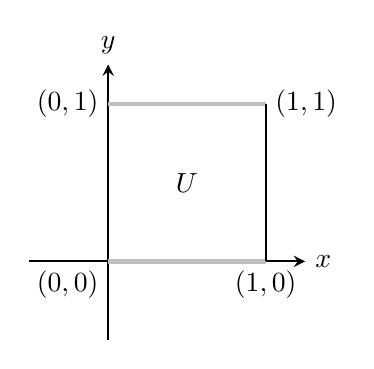
\begin{tikzpicture}
      \def\r{2}
      \coordinate[label=below left:{$(0,0)$}] (A) at (0,0)  ;
      \coordinate[label=below :{$(1,0)$}] (B) at (\r,0);
      \coordinate[label= right:{$(1,1)$}] (C) at (\r,\r);
      \coordinate[label=left:{$(0,1)$}] (D) at (0,\r);
      \draw[thick, -stealth] (-1,0) -- (.5+\r,0) node[anchor=west] {$x$};
      \draw[thick, -stealth] ( 0,-1) -- (0,.5+\r) node[anchor=south ] {$y$};
      \draw[ultra thick, gray!50!white] (A) -- (B) (C) -- (D);
      \draw[thick] (B) -- (C);
      \path (A)--(C) node[midway]{$U$};
    \end{tikzpicture}
    \captionof{figure}{}
    \label{fig:unit-square}
  \end{minipage}
\end{problem}

\begin{subproblem}[2]
  List the ordered pairs in the equivalence classes
  %
  \begin{equation}
    [(0.3, 0.7)], [(0.5, 0)], [(0.4, 1)], [(0, 0.6)], [(1, 0.2)]
  \end{equation}
  %
  For $0 \leq a \leq 1$, $0 \leq b \leq 1$, how many ordered pairs are in $[(a,b)]$?
\end{subproblem}
  
\begin{answer}
  \noindent
  In general if $0 < a < 1$ then $[(a,b)] = {(a,b)}$; otherwise $[(0,b)] =
  {(0,b), (1, b)} = [(1, b)]$. The geometric intuition of this is that the
  highlighted grey parts in \cref{fig:unit-square} are ``glued'' together. This
  gives the following ordered pairs
  %
  \begin{align*}
    [(0.3, 0.7)] & = \{ (0.3, 0.7)\}
    &&[(0.5, 0)] = \{ (0.5, 0)\} \\
    [(0.4, 1)] &= \{(0.4, 1)\}
    &&[(0, 0.6)] = \{ (0, 0.6), (1, 0.6)\} \\
    [(1,0.2)] &= \{(0, 0.2), (1, 0.2)\}.
  \end{align*}
\end{answer}

\end{document}